%%%%%%%%%%%%%%%%%%%%%%% file template.tex %%%%%%%%%%%%%%%%%%%%%%%%%
%
% This is a general template file for the LaTeX package SVJour3
% for Springer journals.          Springer Heidelberg 2010/09/16
%
% Copy it to a new file with a new name and use it as the basis
% for your article. Delete % signs as needed.
%
% This template includes a few options for different layouts and
% content for various journals. Please consult a previous issue of
% your journal as needed.
%
%%%%%%%%%%%%%%%%%%%%%%%%%%%%%%%%%%%%%%%%%%%%%%%%%%%%%%%%%%%%%%%%%%%
%
% First comes an example EPS file -- just ignore it and
% proceed on the \documentclass line
%% your LaTeX will extract the file if required
%\begin{filecontents*}{example.eps}
%%!PS-Adobe-3.0 EPSF-3.0
%%%BoundingBox: 19 19 221 221
%%%CreationDate: Mon Sep 29 1997
%%%Creator: programmed by hand (JK)
%%%EndComments
%gsave
%newpath
%  20 20 moveto
%  20 220 lineto
%  220 220 lineto
%  220 20 lineto
%closepath
%2 setlinewidth
%gsave
%  .4 setgray fill
%grestore
%stroke
%grestore
%\end{filecontents*}
%%
\RequirePackage{fix-cm}
%
%\documentclass{svjour3}                     % onecolumn (standard format)
%\documentclass[smallcondensed]{svjour3}     % onecolumn (ditto)
%\documentclass[smallextended]{svjour3}       % onecolumn (second format)
\documentclass[twocolumn]{svjour3}          % twocolumn

%
\smartqed  % flush right qed marks, e.g. at end of proof
%
\usepackage{graphicx}
\usepackage{stfloats}
\usepackage{amssymb}
\usepackage{amsmath}
\usepackage{url} 
\usepackage{color}
\usepackage{algorithm}
\usepackage{algorithmic}
\usepackage{graphicx}
%\usepackage{slashbox}
%\usepackage{multicol}
\usepackage{xspace}

\usepackage{natbib}

\usepackage{lineno,hyperref}

\DeclareMathAlphabet{\mathpzc}{OT1}{pzc}{m}{it}

\newcommand{\mathkomma}{\quad ,}
\newcommand{\mathpunkt}{\quad .}
\newcommand{\Real}{{\mathbb R}}

\def\etc{etc.\@\xspace}
\def\eg{e.g.\@\xspace}
\def\ie{i.e.\@\xspace}

\newcommand{\red}[1]{\textcolor{red}{#1}}

%
% \usepackage{mathptmx}      % use Times fonts if available on your TeX system
%
% insert here the call for the packages your document requires
%\usepackage{latexsym}
% etc.
%
% please place your own definitions here and don't use \def but
% \newcommand{}{}
%
% Insert the name of "your journal" with
% \journalname{myjournal}
%
\begin{document} \sloppy


\title{Library of Actions: Implementing Human-like Manipulation Actions based on Semantic Event Chains}


%\subtitle{Do you have a subtitle?\\ If so, write it here}

\titlerunning{Library of actions}         % if too long for running head

\author{  Mohamad Javad Aein      \and  	 Florentin  W\"org\"otter	 \and  Eren Erdal Aksoy  	 }

%\authorrunning{Short form of author list} % if too long for running head

\institute{   M. J. Aein,  		F.~W\"org\"otter , E.~E.~Aksoy  \at
              Georg-August-Universit\"at G\"ottingen, BCCN, \\Department for Computational Neuroscience,
              Inst. Physics-3 \\ Friedrich-Hund Platz 1, D-37077 G{\"o}ttingen, Germany \\
              \email{[maein,worgott,eaksoy]@gwdg.de}           %  \\
%             \emph{Present address:} of F. Author  %  if needed
%           \and
%           S. Author \at
%              second address
}

\date{Received: date / Accepted: date}
% The correct dates will be entered by the editor

\maketitle

%%%%%%%%%%%%%%%%%%%%%%%%%%%%%%%%%%%%%%%%%%%%%%%%%%%%%%%%%%%%%%%%%%%%%%%%%%%%%%%%%%%%%%%%%%%%%%%%%%%%%%%%%%%%%
\begin{abstract}

In this paper a new implementation of the library of actions is presented.
Library of actions is a software application which implements  manipulation actions on robotic systems using the semantic event chain framework.
A general definition for manipulation actions is presented which contains both in symbolic and sub-symbolic components.
To connect these two domains, a finite state machine is presented to execute manipulation actions.
The actions are performed both individually and chained sequentially to perform more complex scenarios.
This opens the possibility to use higher-level planners that work in symbolic domain.
The results show that the proposed methodology and software are capable of performing useful human-like actions.


\keywords{Library of Actions \and Execution \and Manipulation Action \and  Semantic Event Chain}
 
% \PACS{PACS code1 \and PACS code2 \and more}
% \subclass{MSC code1 \and MSC code2 \and more}
\end{abstract}


%%%%%%%%%%%%%%%%%%%%%%%%%%%%%%%%%%%%%%%%%%%%%%%%%%%%%%%%%%%%%%%%%%%%%%%%%%%%%%%%%%%%%%%%%%%%%%%%%%%%%%%%%%%%%
\section{Introduction}


Humans are  ..
 
The rest of the paper is organized as follows. We start with introducing the state of the art. We then continue with a detailed description of each processing step. Next, we provide experimental results on various datasets and finally we finish with a discussion.

The rest of the paper is organized as follows.
The high-level action definition is presented in section.\ref{sec:high-level}.
The components of actions in the low-level are introduced in Section.\ref{sec:low-level}.
Section.\ref{sec:Implementing} presents the implementation of actions in the library.
The results of the experiments are shown in Section.\ref{sec:results} followed by some conclusions in Section.\ref{sec:conclusion}.




%\newpage  %% needed for single columns
%\clearpage  %% needed for two columns
%%%%%%%%%%%%%%%%%%%%%%%%%%%%%%%%%%%%%%%%%%%%%%%%%%%%%%%%%%%%%%%%%%%%%%%%%%%%%%%%%%%%%%%%%%%%%%%%%%%%%%%%%%%%%
\section{State of the Art}
\label{sec:soa}
 

%%%%%%%%%%%%%%%%%%%%%%%%%%%%%%%%%%%%%%%%%%%%%%%%%%%%%%%%%%%%%%%%%%%%%%%%%%%%%%%%%%%%%%%%%%%%%%%%%%%%%%%%%%%%%
\section{Method}
\label{sec:method}

Before describing the complete framework in detail, we will briefly provide an overview of each algorithmic step illustrated in Fig.~\ref{fig:block_diagram}.
 

%%%%%%%%%%%%%%%%%%%%%%%%%%%%%%%%%%%%%%%%%%%%%%%%%%%%%%%%%%%%%%%%%%%%%%%%%%%%%%%%%%%%%%%%%%%%%%%%%%%%%%%%%%%%%
\subsection{Manipulation Observation}
\label{sec:observation}
 


%%%%%%%%%%%%%%%%%%%%%%%%%%%%%%%%%%%%%%%%%%%%%%%%%%%%%%%%%%%%%%%%%%%%%%%%%%%%%%%%%%%%%%%%%%%%%%%%%%%%%%%%%%%%%
\subsection{Segmentation and Tracking}
\label{sec:segmentationandtracking}
 

%%%%%%%%%%%%%%%%%%%%%%%%%%%%%%%%%%%%%%%%%%%%%%%%%%%%%%%%%%%%%%%%%%%%%%%%%%%%%%%%%%%%%%%%%%%%%%%%%%%%%%%%%%%%%
\subsection{Semantic Event Chain (SEC) Extraction}
\label{sec:secs}
 

%%%%%%%%%%%%%%%%%%%%%%%%%%%%%%%%%%%%%%%%%%%%%%%%%%%%%%%%%%%%%%%%%%%%%%%%%%%%%%%%%%%%%%%%%%%%%%%%%%%%%%%%%%%%%
\subsection{Learning of Model SECs}
\label{sec:learning}
 
  
  
%%%%%%%%%%%%%%%%%%%%%%%%%%%%%%%%%%%%%%%%%%%%%%%%%%%%%%%%%%%%%%%%%%%%%%%%%%%%%%%%%%%%%%%%%%%%%%%%%%%%%%%%%%%%%
%%%%%%%%%%%%%%%%%%%%%%%%%%%%%%%%%%%%%%%%%%%%%%%%%%%%%%%%%%%%%%%%%%%%%%%%%%%%%%%%%%%%%%%%%%%%%%%%%%%%%%%%%%%%%
%%%%%%%%%%%%%%%%%%%%%%%%%%%%%%%%%%%%%%%%%%%%%%%%%%%%%%%%%%%%%%%%%%%%%%%%%%%%%%%%%%%%%%%%%%%%%%%%%%%%%%%%%%%%%


\section{High-level Action Definition}
\label{sec:high-level}
In this section we give a high-level definition of manipulation actions.
At this level, definitions are mainly symbolic, abstract and close to human description.

A simple action like putting a bucket on a box may be described by a human as following:
\begin{enumerate}
  \item \textbf{\textit{Approach}} the bucket
  \item \textbf{\textit{Grasp}} the bucket
  \item \textbf{\textit{Put}} the bucket on the box
  \item \textbf{\textit{Release}} the bucket
\end{enumerate}
This description is by no means unique.
One could easily describe the same action in different words, with different number of steps and different details.
However, one could still extract some properties from this simple description:
\begin{itemize}
  \item \textbf{Property 1:} The definition is valid even if the objects are changed.
  \item \textbf{Property 2:} An action can be broken into a sequence of smaller sub-actions such as \textit{approach} and \textit{grasp}.
  \item \textbf{Property 3:} There are conditions to end one sub-action and start the next. In the above example these conditions are rather implicit.
  \item \textbf{Property 4:} As humans, we roughly know how to perform these sub-actions.
  Although, our exact movements are produced when we see the objects and perform the action.
\end{itemize}


Our approach to execute human-like actions with robots is similar to this simple example.
We will define a high-level definition of actions which does not depend on the specific objects used in the action (Property 1),
and consists of a sequence of sub-actions (Property 2).
The conditions to start and end each sub-action are defined explicitly (Property 3).
We will store the default trajectory parameters to execute actions in the high-level definition.
When the real objects are seen at each specific instance of the action, these parameters are used to generate the movements (Property 4).


This high-level symbolic definition has several components which will be described in the rest of this section.
For the put-on-top example, the resulting components are shown in fig.\ref{fig:action_graph_sec}.
This definition is an extension to our previous works on the ontology of actions \cite{TAMD13}, semantic event chains (SEC) \cite{Aksoy11b},
and first version of our action library \cite{aein2013toward}.
\begin{figure*}
      \centering
      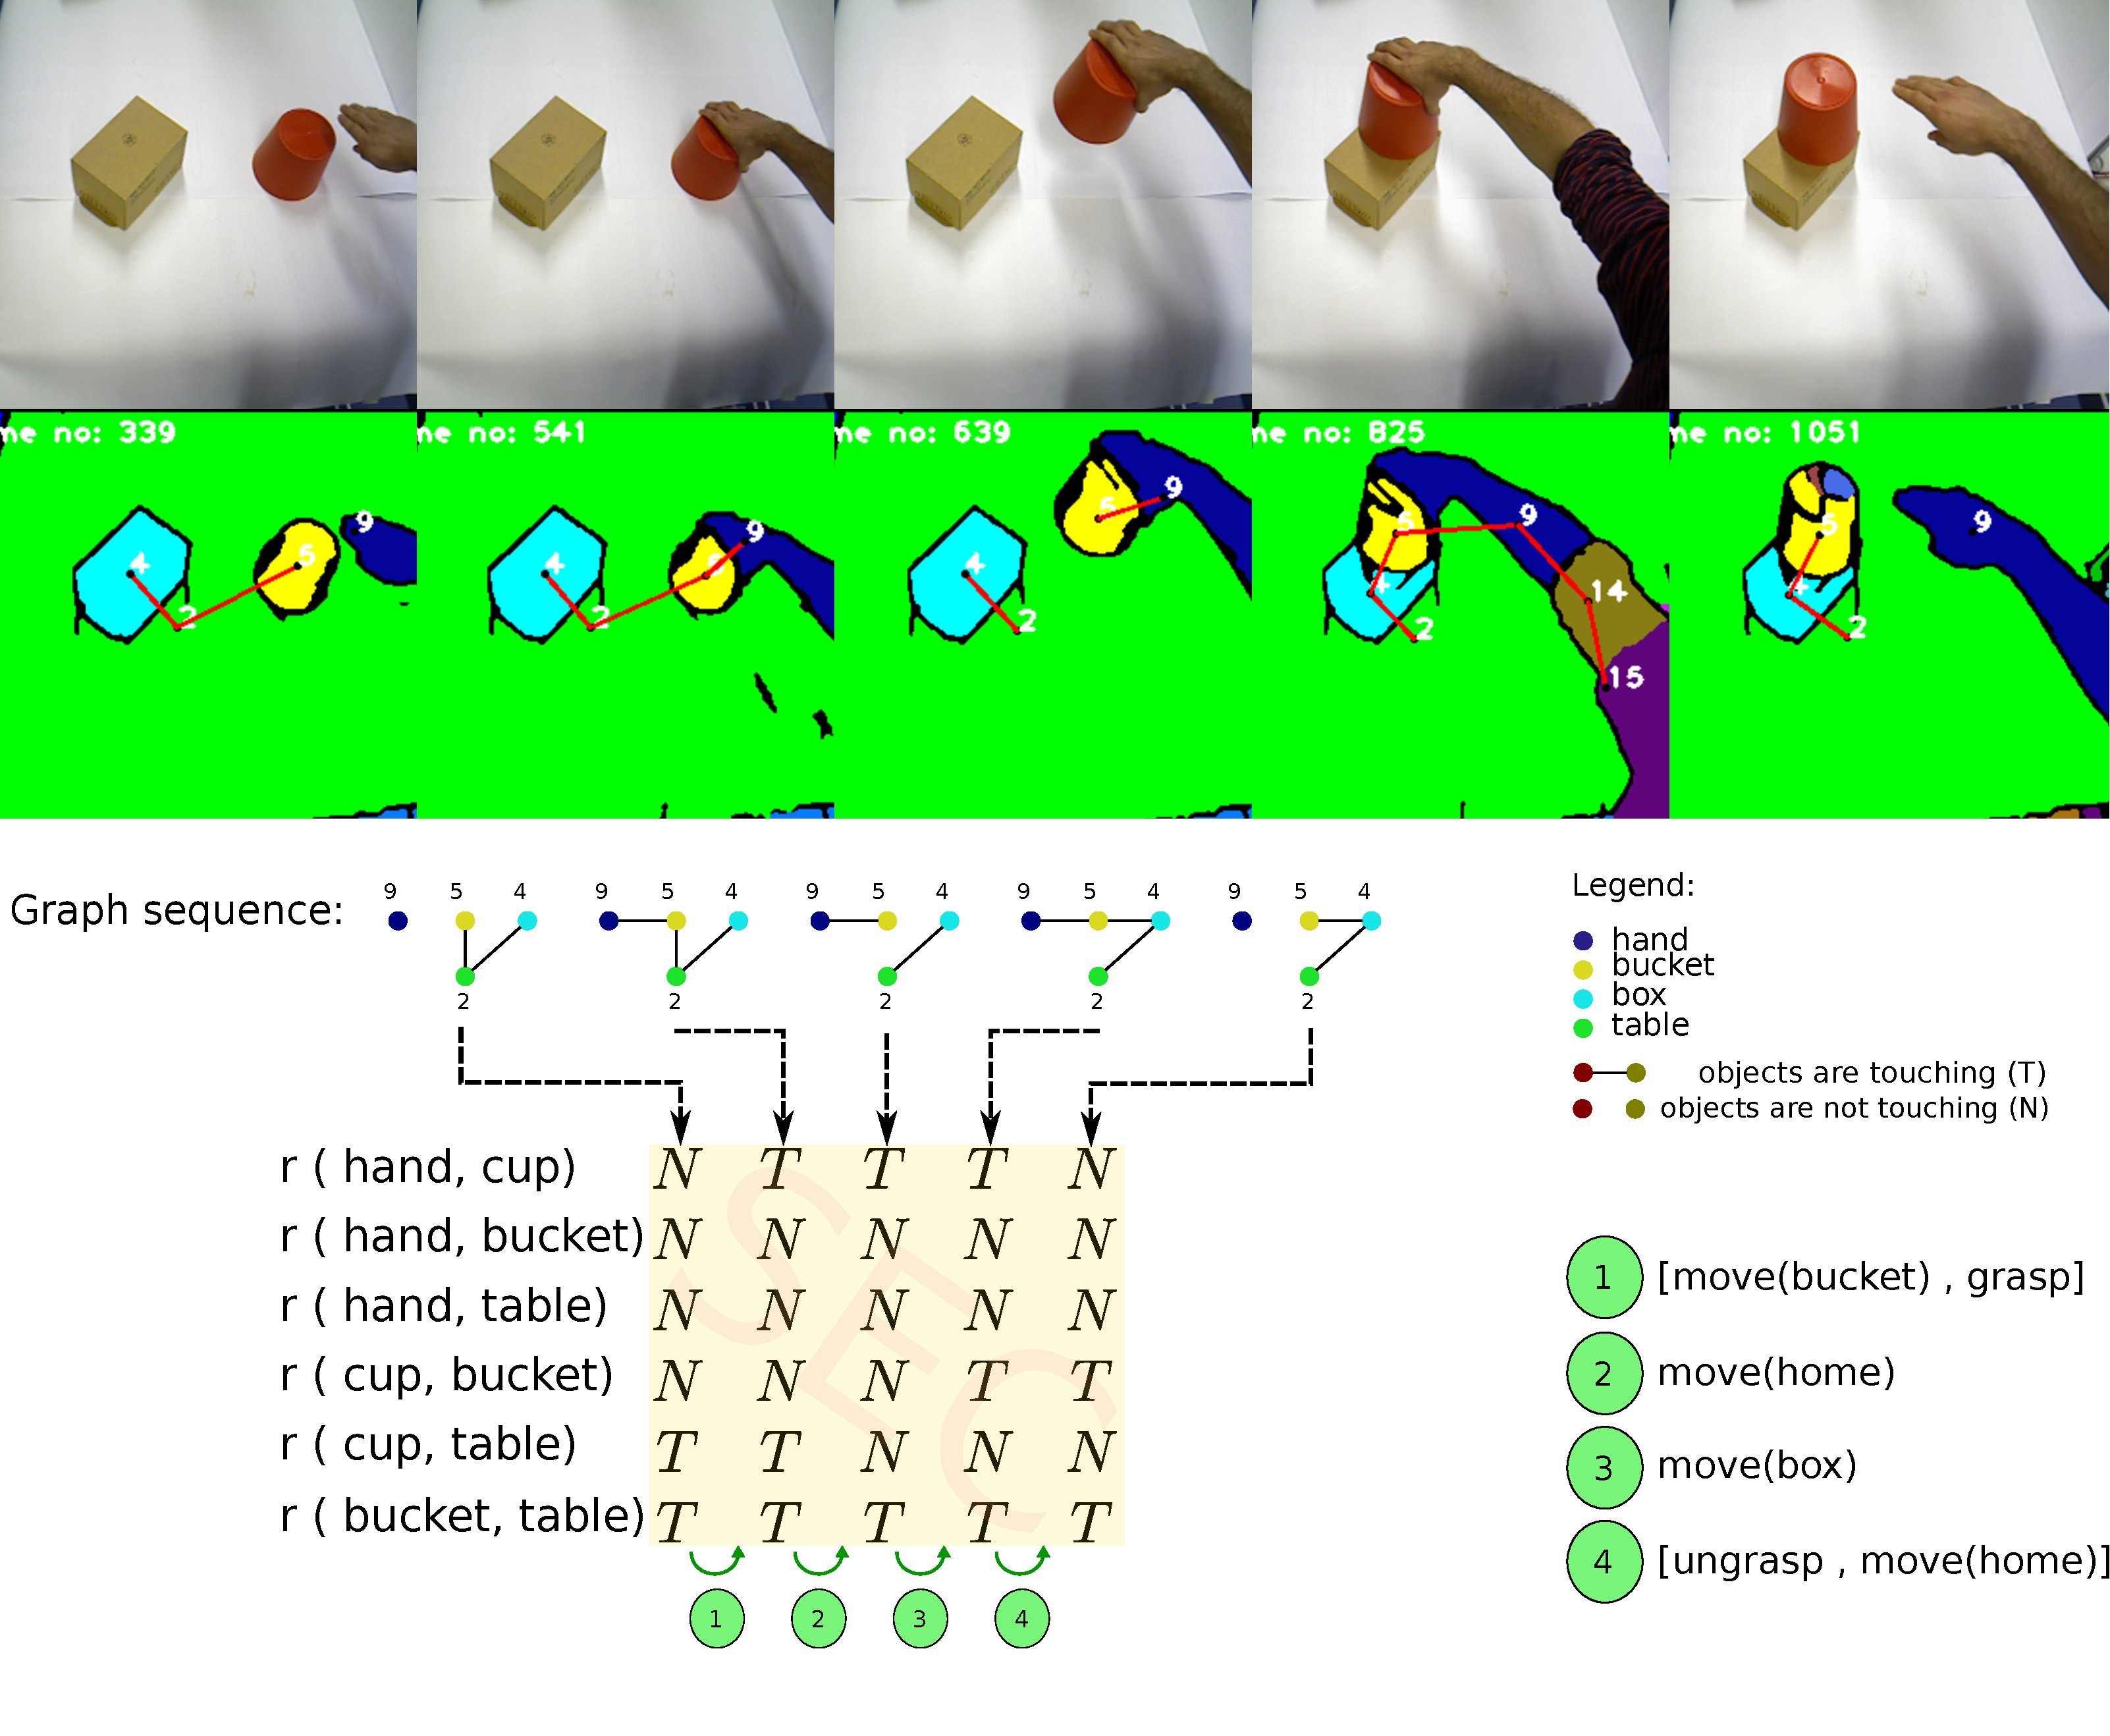
\includegraphics[scale=0.20]{./pdf/action_graph_sec.pdf}
      \caption{ An example of the put-on-top action is performed by a human. 
The snapshots of the executed actions together with segmented images are shown (top).
The symbolic graph sequence (middle) and the SEC matrix (bottom) together with 
the required primitives (bottom right) give a high-level definition of the action.
The abstract objects, manipulator, primary object, secondary object and background are the hand, the bucket, the box and the table, respectively.}
      \label{fig:action_graph_sec}
\end{figure*}

\subsection{Ontology of Actions}
\label{sec:ontology}
The \textit{ontology of manipulation actions} \cite{TAMD13} defines human-like manipulation actions in an abstract way.
An action is defined as change of touching relations between pairs of objects.
The hypothesis is that the most important information are encoded in touching relation of objects.
An example put-on-top actions which is performed by human is shown in fig.\ref{fig:action_graph_sec}.
The segmented images and the extracted graph sequence are also shown.
The nodes of the graphs represent objects and presence of an edge indicates that a pair of objects are touching.
The full action is thus summarized by this sequence of graphs.

There are some constraints on the actions defined in this ontology, which are stated as the following rules:
\begin{itemize}
 \item \textbf{Rule 1:} The action must cause some change in the touching relation of objects, including the manipulator (human or robot hand)
 \item \textbf{Rule 2:} The action is performed by one hand. This is true for the most of human actions, since the second hand is usually used as support.
 \item \textbf{Rule 3:} The hand is free at the beginning and at the end of action.
 \item \textbf{Rule 4:} The hand touches one object at the beginning of action and does not purposefully touch another object in the scene.
\end{itemize}

The last constraint is used to make sure that the defined actions can not be split into two simpler actions in the ontology.
There are less than 30 unique actions in the ontology.
For a complete list of the actions and more information we refer to \cite{TAMD13}.

\subsection{Abstract objects}

There are too many objects in the real world.
It is not practical to define each action separately for each object.
It is then necessary to define manipulation actions in a general way so that they are applicable to different objects.
To deal with this problem, we define objects by the role that they play in the action.
First of all, one object is needed that performs the action, which is here called the \textit{manipulator}.
Then, there exists an object that is manipulated directly by the manipulator.
This object is called \textit{primary object}.
For example, in the put-on-top action in fig.\ref{fig:action_graph_sec}, the human hand is the manipulator and the bucket is the primary object.

In some actions there is another object which is indirectly manipulated by the manipulator.
For example if the hand picks up a bucket and puts it on a box, as shown in fig.\ref{fig:action_graph_sec},
the box plays the role of the indirect object or the \textit{secondary object}.
There could be more than one indirect objects in an action, but in this work we will consider actions with one indirect object.

Adding the relation of objects with the background is important in representing and executing the actions (See \cite{TAMD13}).
By adding the background, different graphes emerge for ``one object on top of another object'' and ``one object next to another object''.
Another advantage of adding the background is that it adds an ``air-phase'' to actions,
which happens when one object is lifted and moving on air, but it is not yet touching the other object.

Therefore the last object that we add to the action definition is the \textit{background}.
In our example, the background is the table.
The result is that the number of objects involved in an action is (at most) four: manipulator, primary object, secondary object and background.

\begin{table}
\caption{Abstract relations and their attributes for the put-on-top action}
\begin{tabular}{ lllll }
\hline\noalign{\smallskip}
Relation Name & Abstract Relation & Real Relation & Type \\
\noalign{\smallskip}\hline\noalign{\smallskip}
$\text{R}_1$  & R(manipulator,primary object) & R(hand,bucket) & variable \\
$\text{R}_2$  & R(manipulator,secondary object)& R(hand,box) & don't-care \\
$\text{R}_3$  & R(manipulator,background) & R(hand,table) & don't-care \\
$\text{R}_4$  & R(primary object,secondary object) & R(bucket,box) & variable  \\
$\text{R}_5$  & R(primary object,background) & R(bucket,table) & variable \\
$\text{R}_6$  & R(secondary object,background)& R(box,table) & constant \\
\noalign{\smallskip}\hline
\end{tabular}
\label{tab:relations}
\end{table}

\subsection{Abstract relations}
The relations between objects play the key role in the definition of the actions.
These abstract relations are assigned to pairs of abstract objects (See Table \ref{tab:relations}).
If there exists $N$ objects in an action,
there will be $N(N-1)/2$ distinct relations.
As stated before, there are 4 abstract objects in our defintion, which gives in total 6 abstract relations.


Each relation is defined by two attributes, which are  \emph{type} and \emph{value}.
The \emph{type} of a relation is determined by the importance and variation of that relation throughout the action.
For example for the put-on-top action, the relation between the hand and the table, does not affect the outcome of the action.
The type of such relations is \emph{don't-care}.
The importance of a relation is decided based on common sense.

Other relations, which are important for an action, are divided into \emph{variable} and \emph{constant} relations.
For example, the relation between manipulator(hand) and primary object(bucket) for the put-on-top action is \emph{variable},
whereas the relation between the secondary object(box) and the background(table) is \emph{constant} (see Fig. \ref{fig:action_graph_sec}).
The constant relations show the necessary conditions to perform an action and a change in them implies failure of the action.
On the other hand, variable relations encode the progress of the action and play the most important role in our methodology.

The \emph{value} of a relation is either N (for Not touching), T (for Touching) or A (for absent).
Absent value happens when there is no information about the relation, e.g., one object is not defined or not visible.
Table \ref{tab:relations} shows the abstract relations and their type attributes for the put-on-top action.


\subsection{Semantic Event Chain}
\label{sec:SEC}
The actions in the ontology are defined as sequences of graphs (see Fig.\ref{fig:action_graph_sec}).
The nodes of these graphs are the objects and the edges show the touching relation between a pair of objects.
A semantic event chain (SEC) \cite{Aksoy11} is a matrix derived from these graph sequences.
Each row of the SEC matrix shows changes that occur in one abstract relation.
Since there are six abstract relations, the SEC matrix has 6 rows.
The number of columns of SEC, depends on how many times the relations between objects change in the course of action.
Each column of SEC matrix is interpreted as a state of the scene, which is a combination of the relations between the objects.


The valid symbolic entries of SEC matrix are N (not touching), T (touching) and A ( absence).
In a SEC, the progress of the action from the beginning to the end, is seen in a compact way.
In addition, the SEC matrix of different instances of one action remains the same.
The SEC matrix of the put-on-top action is shown in Fig.\ref{fig:action_graph_sec}.

\subsection{Abstract Primitives}
\label{sec:abstract_primitives}
In the simple example at the beginning of this section, it is shown that a full action can be divided into several sub-actions.
These sub-actions or \textit{primitives} are the basic functions of the manipulator.

In our approach we define the following primitives:
\begin{itemize}
 \item $move(pose)$ :  The manipulator moves to $pose$.
 \item $move_{periodic}(path)$ : The robot arm moves periodically along the given path.
 \item $force()$ : The robot arm exerts $force$.
 \item $grasp()$ : The robot hand grasps an object.
 \item $release()$ : The robot hand releases an object.
\end{itemize}


These primitives are the basic functions of our hardware which can be implemented in many different ways.
The focus of our work is not implementing these primitives,
but rather we would like to propose a way to combine them to produce actions.
Nevertheless, our implementations are presented in section.\ref{section_primitives}.

In Fig.\ref{fig:action_graph_sec}, the necessary primitives associated to each column of the SEC matrix are shown.
There number of primitives at each phase is either one or two.
The reason to add a second primitive is that sometimes more than one primitives are needed to make the desired event i.e. the desired change in the relations.
For example, a combination of $move(pose)$ and $grasp()$ primitives are often necessary to grasp an object.

\subsection{Abstract Positions}

As described above, one important primitive is the $move(pose)$ primitive that moves the robot arm toward a pose.
In the abstract definition, the argument $pose$ of this primitive is an abstract position.
The abstract positions are either the objects in the scene, or some other convenient points in space.
While performing the actions, sometimes we move our hands toward points in space where there are no specific objects.
One example is when we initially lift an object from a table, to put it on top of another object.
We move the object to a point that makes our next move easier.
We call such positions \textit{home}.

In some actions, we need to move toward arbitrary positions to achieve the goal of the action.
For example in the pushing action, we push an object to a desired position.
This desired position could be any accessible point and it is usually specified by the user or a higher level planner.
We call this type of abstract positions the \textit{goal} position.

%%%%%%%%%%%%%%%%%%%%%%%%%%%%%%%%%%%%%%%%%%%%%%%%%%%%%%%%%%%%%%%%%%%%%%%%%%%%%%%%
%%%%% SECTION
%%%%%%%%%%%%%%%%%%%%%%%%%%%%%%%%%%%%%%%%%%%%%%%%%%%%%%%%%%%%%%%%%%%%%%%%%%%%%%%%
\section{Low-level Action Definition}
\label{sec:low-level}
In this section, the abstract components of the high-level definition are related to their real-world counterparts.
This includes defining objects in the real world, implementing the low-level primitives such that proper commands are sent to the hardware control systems,
and calculating the object relations from the sensor data.
In the rest of this section, these steps are described in more detail.

\subsection{Real objects}
In the real world experiments, the abstract objects (\textit{manipulator}, \textit{primary object}, \textit{secondary object} and \textit{background})
are instantiated by real objects in the scene.
For the put-on-top example depicted in Fig. \ref{fig:action_graph_sec},
these objects are manipulator=hand, primary object=bucket, secondary object=box and background=table.
We need to represent the real-world objects in signal space so that we can perform the primitives.

In our work, two pieces of information is needed to represent an object.
First, the position of each object with respect to some fixed frame is needed.
The frame is fixed to the workspace of the robot.
To associate a position to the object, the objects are modeled with a single point, located at their center of mass.
Second, the direction of objects in the XY-plane should be detected.
This is necessary for grasping the objects, as well as some actions like cutting.
Note that we use this direction information only for elongated objects (such as cucumber) but not for symmetric objects (such as apple, cup etc.)
The direction is defined as the angle that the main axis of the object makes with respect to the X-axis of the reference frame.

To this end, we use our vision system to represent each object in the scene with a point cloud.
\textcolor{red}{Eren: a short description of vision system is needed}
Using the point cloud we can calculate the center of mass of the object.
To calculate the direction of the objects, we use principle component analysis (PCA) to find the major axis of the object.
The direction of the object is defined as the direction of its major axis.

\begin{table}
\caption{Summary of object relation detection in different actions. For each relation only the main sensor is mentioned.}
\begin{tabular}{ lcccccc }
\hline\noalign{\smallskip}
 Action Name &  $\text{R}_1$ & $\text{R}_2$ &$\text{R}_3$ &$\text{R}_4$ &$\text{R}_5$&$\text{R}_6$ \\
\noalign{\smallskip}\hline\noalign{\smallskip}
 Pick and Place & tactile & -       & position & -     &  force & - \\
 Put-on-top     & tactile & tactile & position & force &  vision & vision \\
 Take-down      & tactile & tactile & position & vision&  force & vision \\
 Put-in         & tactile & tactile & position & force &  vision & vision \\
 Cut            & tactile & tactile & position & force &  position & vision \\
 Unload         & tactile & tactile & position & vision&  force & vision \\
 Stir           & tactile & -       & position & vision&  vision & - \\
 Push           & force   & -       & position & -     &  vision & - \\
 Poke           & force   & -       & position & -     &  vision & - \\
\noalign{\smallskip}\hline
\end{tabular}
\label{tab:relation_detection}
\end{table}
\subsection{Real relations}
\label{sec:real_relations}
The real relations are the actual relations between pairs of objects.
These relations together form a symbolic representation of the scene, or in other words, the current state of system.
To detect the relations, we use combination of vision, position, force and tactile sensors.

When it comes to detecting the object relations, there are three distinct phases: before the action, during the action and after the action.
In the first and last phases, the main source of information is the vision system.
In the middle phase , when the action is being performed, the sensors of the robot play the main role,
and the vision system acts as a support to confirm the outcome of these sensors.

At the beginning and the end of the action, we have some objects located on a background, and a manipulator which is away from the objects.
This is a result of the Rule.3 (see Section.\ref{sec:ontology}) in the ontology.
This requires the first three relations (the relation of manipulator with the objects and the background) to be equal to N.
The vision system can detect that we are in a proper state.
The tactile sensors of the robot hand are also used to confirm that no object is grasped by the hand.
The last three relations can only be detected by vision.
These are the relations of the primary object, the secondary object and the background.

During the action, the relations of the objects are calculated by combining data from different sensors.
The sensors used for each relation and how the data from different sensors are combined, depends on the type of the action.
Next we describe how these relations are calculated in the put-on-top action.

The relation of the manipulator with the primary and secondary objects are calculated from the position and tactile sensors.
When the position of the manipulator is close to the \textit{primary} (\textit{secondary}) object and the tactile sensors sense that the manipulator has grasped something,
$\text{R}_1$ ($\text{R}_2$), is changed to T.
Although we can detect the $\text{R}_2$, usually this relation is not important and marked as don't-care.
The reason is that the manipulator does not directly interact with the secondary object.

The relation of the manipulator and the background ($\text{R}_3$) plays no important role in this action, so we label it as don't-care.
This is not specific to this action and for all other actions the $\text{R}_3$ is don't-care.


The relation of the primary object and the secondary object ($\text{R}_4$) is calculated by force sensor of the robot arm.
However, this depends also on the relation of manipulator and primary object, and on the position sensor.
In short, when the manipulator holds the primary object and it approaches the secondary object,
if the force sensor reads a contact force in the opposite direction of movement, the relation is changed to touching (T).
The position sensor is used to confirm that the relative pose of the objects is correct and they are close enough for a contact.
The relation of primary object and the background ($\text{R}_5$) is also detected in a similar way.

The relation of the secondary object and the background ($\text{R}_6$) is a constant relation and is detected by vision.
For the cases that other sensors than vision are used, the vision sensor is also employed to confirm the resulting event.
The sensors used to detect relations during different actions are summarized in table.\ref{tab:relation_detection}.

\subsection{Low-level primitives}
\label{section_primitives}
In section.\ref{sec:abstract_primitives} we defined the primitives which are performed by the manipulator.
Here we describe our implementation of these primitives at the low-level.

For the robot arm, we have three primitives: $move(p_{des},P)$, $move_{periodic}(W)$ and $exert(F)$.
The first two primitives generate trajectories for the position control of the robot.
To generate the trajectories in the Cartesian space, we use dynamic movement primitives (DMP) with joining introduced in \cite{Kulvicius2012}.
The argument $P$ represents the parameters of the DMP which consist of parameters of Gaussian kernels and the time of trajectory $T$.
The parameters of the kernels are the number $n$, width $\sigma$ and weights $W$.
The details of implementation are not covered here, but the final result is that by using the primitive $move(p_{des},P)$
we can move the robot arm from the current position and orientation, to any desired position and orientation, along the desired trajectory.

The $exert(f_{des},P)$ performs force control with set-point $f_{des}$.
In our setup, we use a parallel force/position scheme with dominant force control, similar to \cite{chiaverini1993parallel}.
In this way we can achieve the desired force in the constrained space, and at the same time, perform desired motions in the unconstrained space,
the trajectory of which is defined by $P$.


To grasp objects we use velocity control of finger joints together with feedback from tactile sensors on the fingers.
We use separate pre-shapes for round and elongated objects.
This provides grasps for simple objects, which is enough to demonstrate our system.
The complex problem of grasping arbitrary objects is not a goal of this research.

%%%%%%%%%%%%%%%%%%%%%%%%%%%%%%%%%%%%%%%%%%%%%%%%%%%%%%%%%%%%%%%%%%%%%%%%%%%%%%%%
%%%%% SECTION
%%%%%%%%%%%%%%%%%%%%%%%%%%%%%%%%%%%%%%%%%%%%%%%%%%%%%%%%%%%%%%%%%%%%%%%%%%%%%%%%
\section{Implementing the Actions}
\label{sec:Implementing}

In this section we present our implementation of manipulation actions based on the high-level and low-level definitions given in the previous sections.
First we introduce the hardware setup used in the experiments.
Then, we present the software components that are developed as part of the library of actions.
Finally, our algorithm for executing actions is described as a finite state machine.



\subsection{Hardware}
\label{sec:hardware}
The action library is designed to execute actions on a general robotic arm/hand system.
Here we describe the hardware in our setup as used in the experiments in section \ref{sec:results}.
Our setup consists of a 7-DOF KUKA LWR robot manipulator, a three-fingered robotic hand and a vision system. 
The vision system is a RGB-D camera. \textcolor{red}{Eren: please rewrite this sentence if necessary.}

\subsubsection{Robot Arm}
Our robot arm is a KUKA LWR (Light Weight Robot) IV manipulator.
It is a kinematically redundant anthropomorphic manipulator developed jointly by KUKA Robot Group and the German Aerospace Center (DLR).
It has 7 DOFs and is equipped with position and torque sensors at each joint.
It estimates the external torques applied to each joint which also gives an estimate of external force and torque at the end effector.
The robot can be commanded both in joint space and Cartesian space, with variable compliance and damping.

By using a C++ library called the Fast Research Interface (FRI) it is possible to communicate to LWR's control system and sensors, from an external PC.

\subsubsection{Robot Hand}
Our robot hand is a SDH-2 (Schunk Dexterous Hand 2) produced by the Schunk company.
It has three fingers and 7 degrees of freedom, which can be controlled in position or velocity modes.
It has tactile sensors that provide feedback when grasping objects.

\subsubsection{Vision System}
Our vision system includes an RGB-D camera (Microsoft Kinect) and a DSLR camera.
\textcolor{red}{Eren: please develop this part}

\subsection{Software}
\label{sec:software}
The library of actions is implemented as an application in the Open Robot Control Software (Orocos) framework \cite{rtt-url,soetens2006}.
The Orocos is a framework to develop real-time robotic and automation applications.
In a typical Orocos application, several components exist which communicate over (possibly real-time) data ports.
The library of actions consists of several components which are shown in fig.\ref{fig:software_structure}.
Some of the components communicate to hardware (Sensors and actuators), while others perform calculations and control the execution of actions.
The components are described in the following:
\begin{figure*}
      \centering
      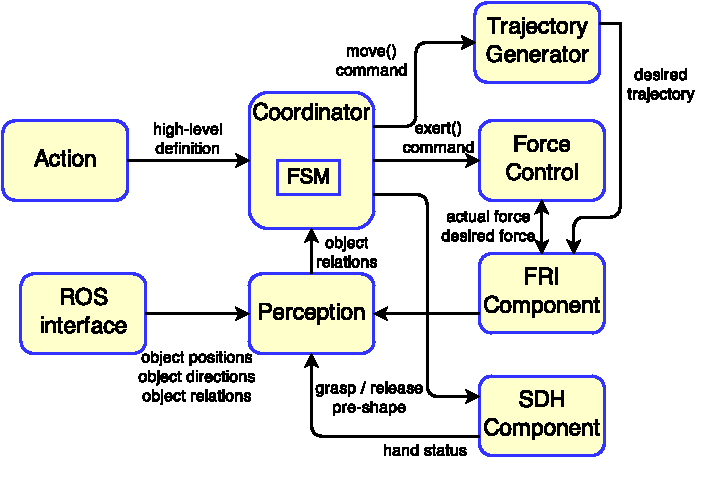
\includegraphics[scale=1]{./pdf/software_structure.pdf}
      \caption{ Block diagram of the software for action library.
      The interconnection of the components are shown as well as the interface to ROS nodes and hardware.
}
      \label{fig:software_structure}
\end{figure*}



\begin{itemize}
 \item{\textbf{Action}}
component holds the parameters of the high-level definition of the action.
These parameters are the SEC matrix, high-level primitives and the abstract arguments.
The parameters of the DMP for trajectories are also stored in this component.
\item{\textbf{Perception}}
component collects data from all the sensors and determines if the relations of objects in the scene are altered.
It receives the object poses from the vision system (through the ROS-interface component).
It also monitors other sensors and detects changes in object relations according to section.\ref{sec:real_relations}.
\item{\textbf{Coordinator}}
component contains a state machine that executes the action.
The detail of the state machine and execution algorithm will be discussed in \ref{sec:execution_algorithm}.
Additionally, some function like comparing desired and actual relations is done inside this component.

\item{\textbf{Trajectory Generator}}
component receives $move()$ and $move_{periodic}()$ primitives and generates the trajectory using the DMPs.

\item{\textbf{Force Control}}
component implements the $exert()$ primitive.
The actual contact force is received from the FRI component and using the algorithm of section.\ref{section_primitives},
the contact force is regulated in the desired direction.
The output of this component is sent to the control system of the LWR arm, though the FRI component.

\item{\textbf{FRI}}
component communicates with the robot arm through the FRI,
and provides the necessary input and output data ports to other Orocos components.

\item{\textbf{SDH}}
component implements the hand primitives (grasp, release and pre-shape).
This component uses the C++ library which is provided to communicate with the Schunk SDH-2 robot hand.
The tactile sensor data are also processed in this component to detect objects in the hand.
The parameter $hand\_status$ determines the current status of the hand and is sent to the perception component.
This parameter takes values : Undefined, Grasped and Empty

\item{\textbf{ROS interface}}
component creates an interface between the ROS nodes and Orocos data ports.
The data ports in Orocos are capable of talking to ROS nodes, using the components of $rtt\_ros\_integration$ stack.
% \footnote{http://wiki.ros.org/rtt_ros_integration}.
This component is created using the $rtt\_rosnode$ component of this stack to integrate all ROS communications in one component.
Since our vision system is developed in ROS framework, this component is used to get the information such as 
objects poses and relations from the vision system and create the necessary data ports to send them to other components.
\end{itemize}

\subsection{Execution Algorithm}
\label{sec:execution_algorithm}
\begin{figure*}
      \centering
      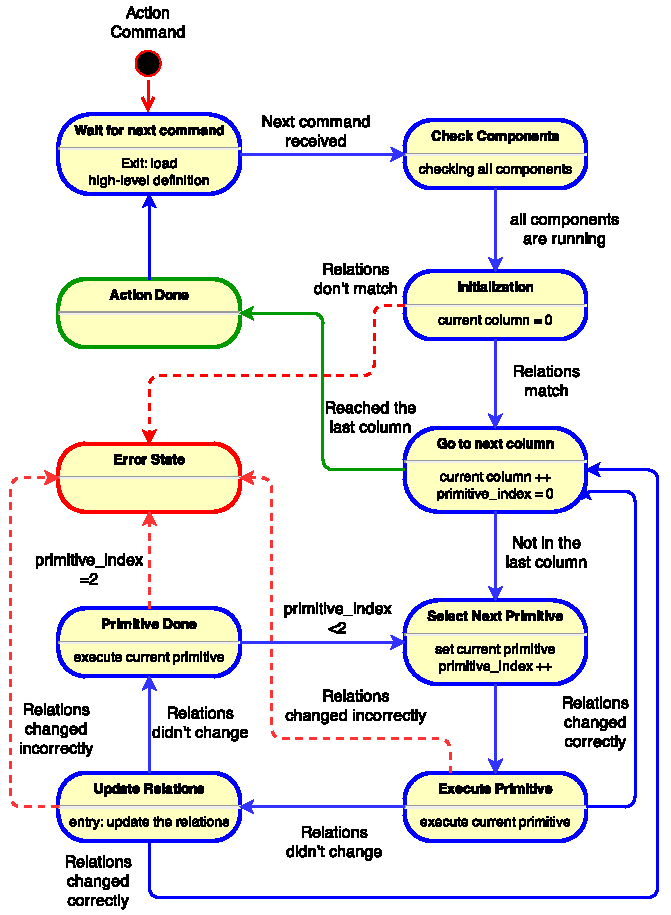
\includegraphics[scale=1]{./pdf/coordinator_fsm.pdf}
      \caption{ State diagram of the finite state machine governing the execution of action.
}
      \label{fig:coordinator_fsm}
\end{figure*}
Here an algorithm is presented to execute actions, using the software components introduced earlier.
The core of the execution is a finite state machine inside the coordinator component.

To implement the state machine, we use the $State\_Machine$ class in Orocos real-time toolkit (RTT).
The Orocos component builder manual defines a state machine:
``A state machine is composed of a set of states. A running state machine is always in exactly one of its states.
One time per period, it checks whether it can transition from that state to another state, and if so makes that transition.
It contains a collection of states, and each state defines a Program on entry of the state, when it is run and on exit.
It also defines all transitions to a next state.''

The diagram in figure.\ref{fig:coordinator_fsm} shows the designed state machine that controls the execution of actions.
The states are described in detail in the following:
\begin{itemize}
 \item \textbf{Wait for next command:} Waiting for the next action command to come.
 An action command consists of the action type, the primary object and the secondary object.
 On exit, the high-level definition of the requested action is loaded in the action component.
 \item \textbf{Check components:} This state checks whether all the components are running and ready to execute the action. 
 \item \textbf{Initialization:} This component initializes the $curren\_column$ parameter to zero.
 This means that the action starts at the first column of the SEC matrix.
 Then the current relations are compared to the first column of SEC matrix.
 If they match, the initialization is successful and a transition is made to \textit{Go to next column} state.
 Otherwise the action is aborted at the beginning, since the initial conditions are not correct, and the system transitions to the \textit{Error} state
 \item \textbf{Go to next column:} In this state, the desired relations are changed to the next column of SEC matrix,
 assuming that the current relations are equal to the current column of the SEC matrix.
 To do this, the variable $current\_column$ is incremented.
 The variable $primitive\_index$ is reset to zero. This means that the first primitive should be executed.
 If $current\_column$ is already pointing to the last column of the SEC matrix, it makes a transition to $Action\ done$ state.
 \item \textbf{Select next primitive:} Based on the high-level action definition and the $primitive\_index$,
 the next primitive to be executed is selected here.
 \item \textbf{Execute primitive:} The selected primitive is executed here.
 This state has several sub-states, each performing one type of primitive.
 To keep the diagram simple, they are not shown in Fig.\ref{fig:coordinator_fsm}.
 During execution, the actual relations are monitored.
 If the relations match the desired relations while the primitive is being executed, a transition to $Go\ to\ next\ column$ is issued.
 If the relations are changed to the wrong values, the next state will be the $Error$ state.
 If the relations don't change, we move to the $Update\ relations$ state to evaluate the outcome of the primitive.
 
 \item \textbf{Update relations:} At this state, the relations are once more updated to see if the desired changes in states has occurred.
 If this is the case, we move to the $Go\ to\ next\ column$ state.
 Otherwise, we move to the $Primitive\ finished$ state.
 \item \textbf{Primitive finished:} This state is reached when a primitive is finished but the relations are not changed to the desired values.
 If there is another primitive to execute, a transition is made to the $Select\ next\ primitive$ state.
 If there is no more primitive to do, the $Error$ state is selected, as this indicates an error in the execution.
 \item \textbf{Action done:} This state is entered if the action is successfully executed according to the SEC matrix.
 After this state we transit to the $Wait\ for\ next\ command$ state, so that the next action is executed.
 \item \textbf{Error:} This state shows that the execution of the action is not progressing as expected.
 This could be used to inform the user or the higher level planner that the action is not successful.
\end{itemize}


%%%%%%%%%%%%%%%%%%%%%%%%%%%%%%%%%%%%%%%%%%%%%%%%%%%%%%%%%%%%%%%%%%%%%%%%%%%%%%%%
%%%%% SECTION
%%%%%%%%%%%%%%%%%%%%%%%%%%%%%%%%%%%%%%%%%%%%%%%%%%%%%%%%%%%%%%%%%%%%%%%%%%%%%%%%
\begin{figure*}
      \centering
      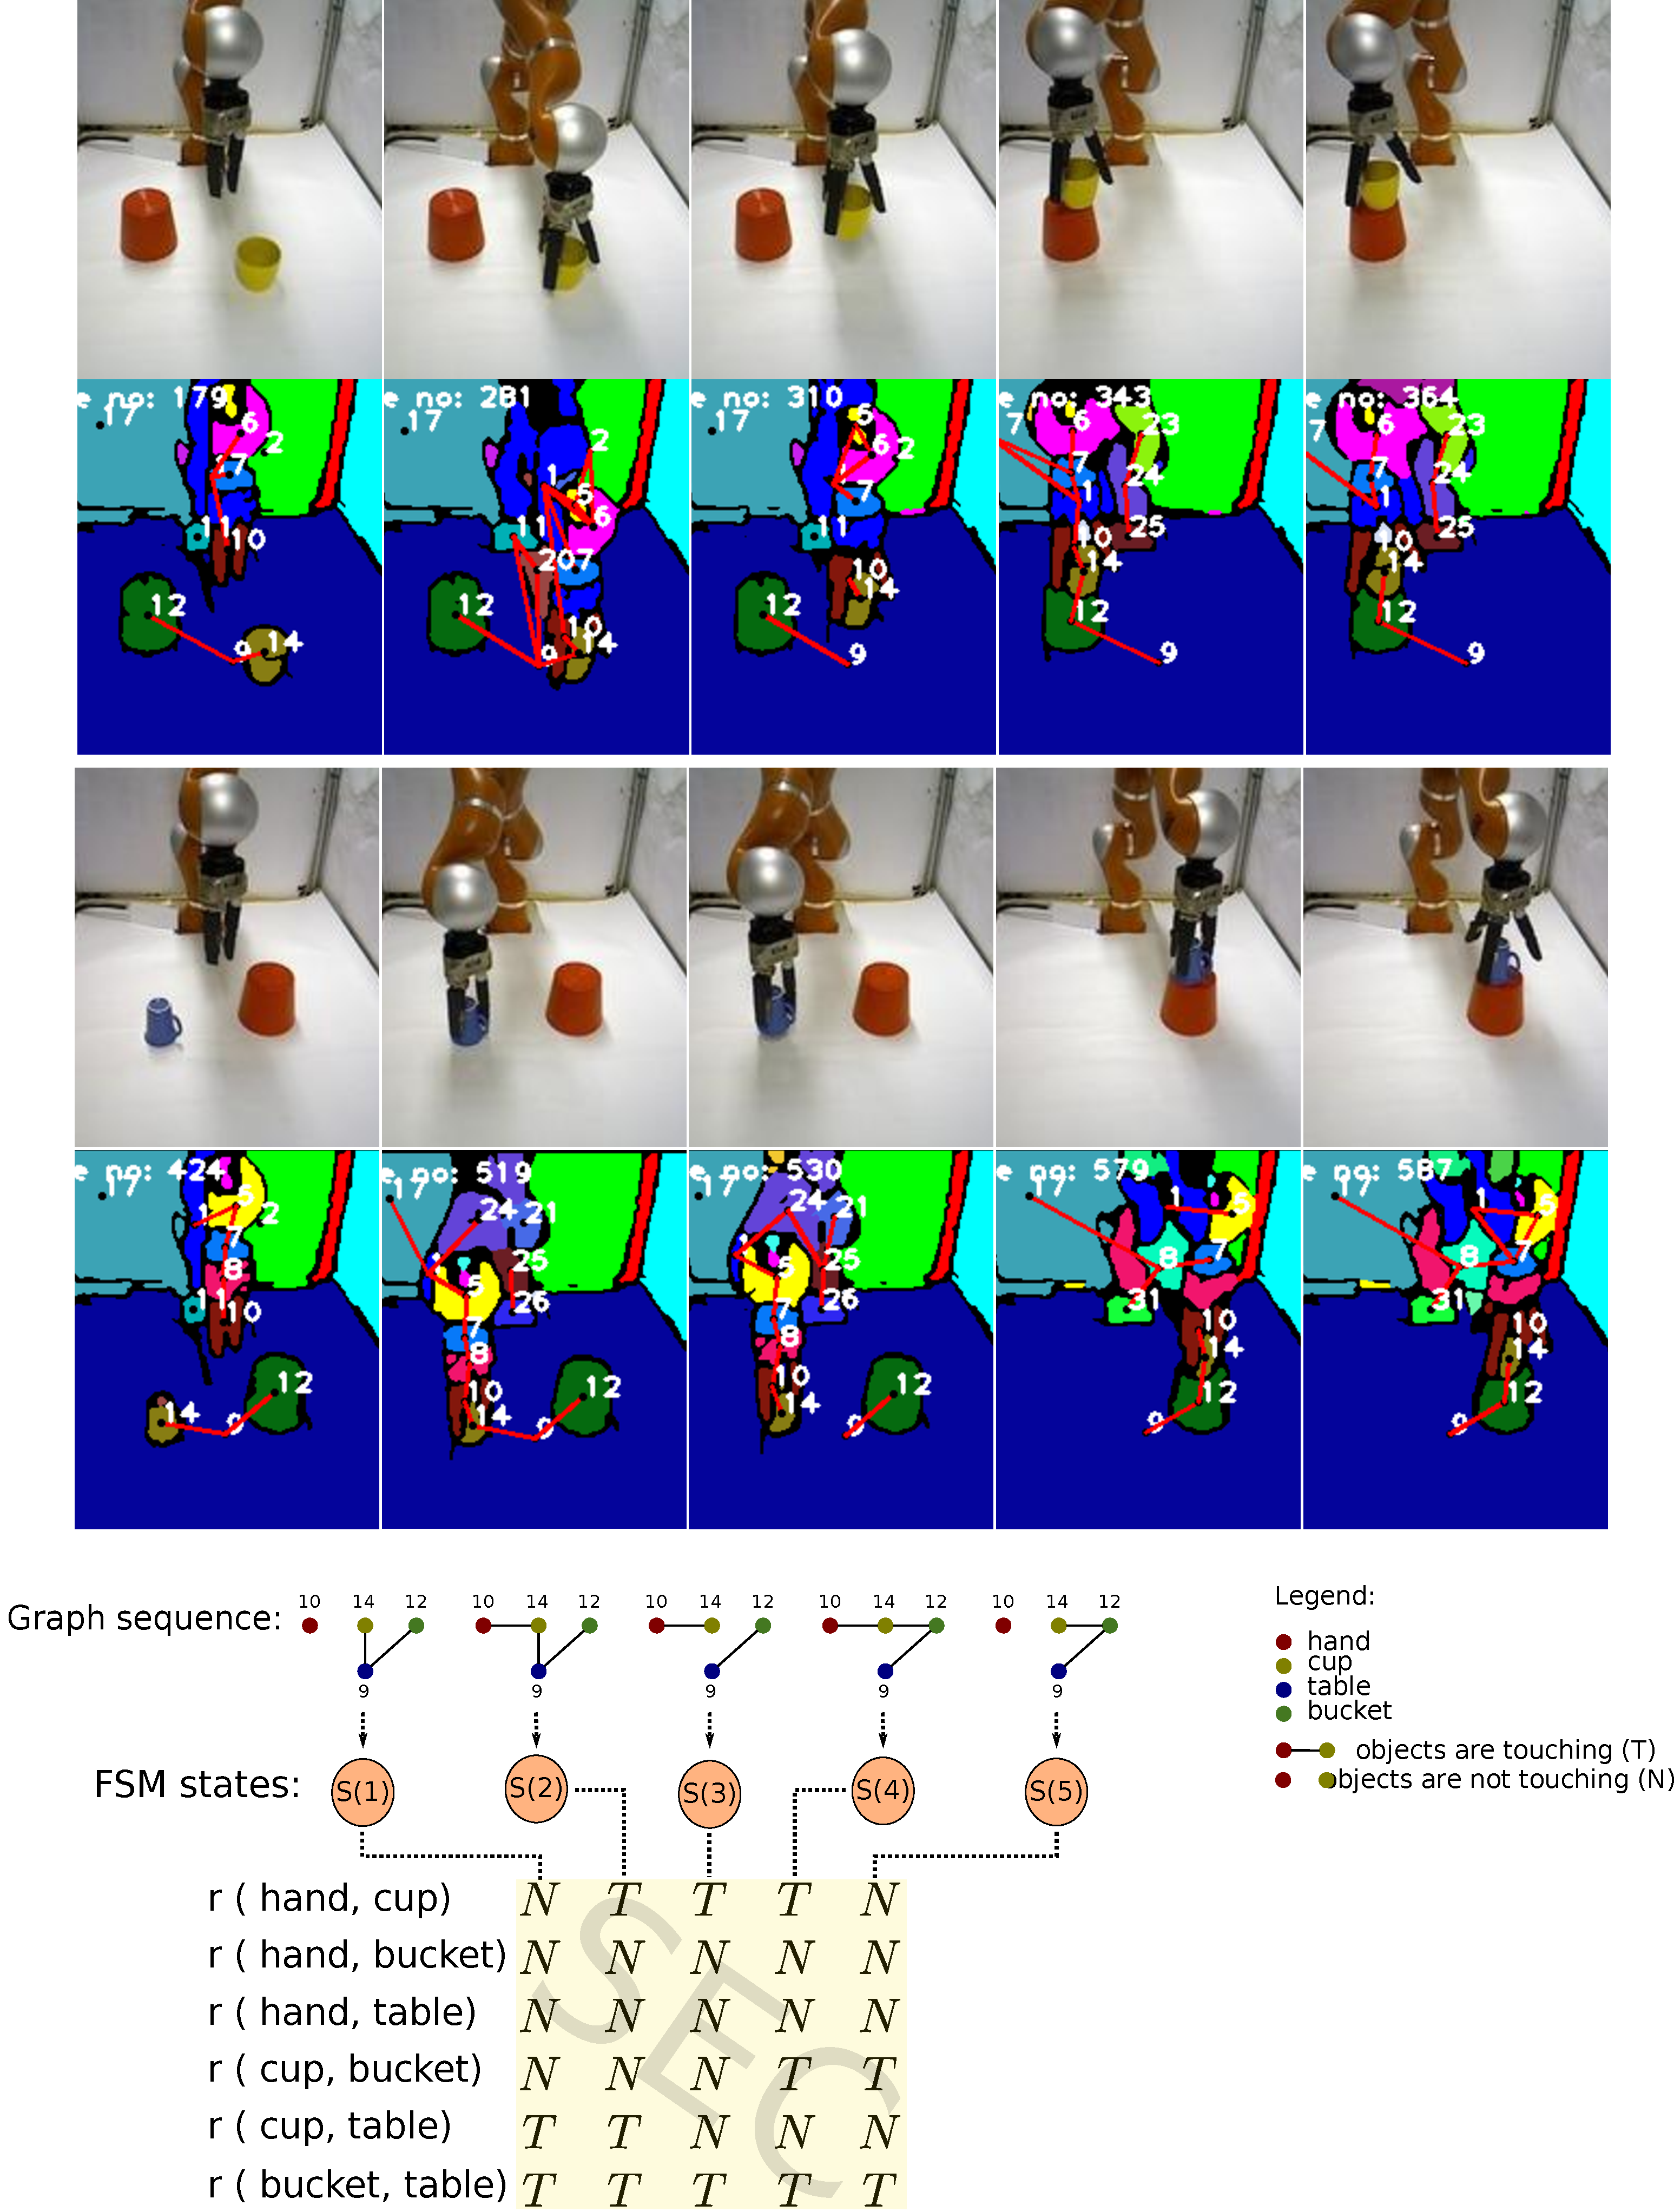
\includegraphics[scale=0.20]{./pdf/result_puton.pdf}
      \caption{ Two instances of the put-on-top action, performed by our method, are shown with different objects and positions. 
The snapshots of the executed actions together with segmented images are shown (top) which indicate the real objects and relations.
The symbolic graph sequence (middle) and the SEC matrix (bottom) remain the same for both version.
}
      \label{fig:result_puton}
\end{figure*}
\section{Results}
\label{sec:results}

\begin{figure*}
      \centering
      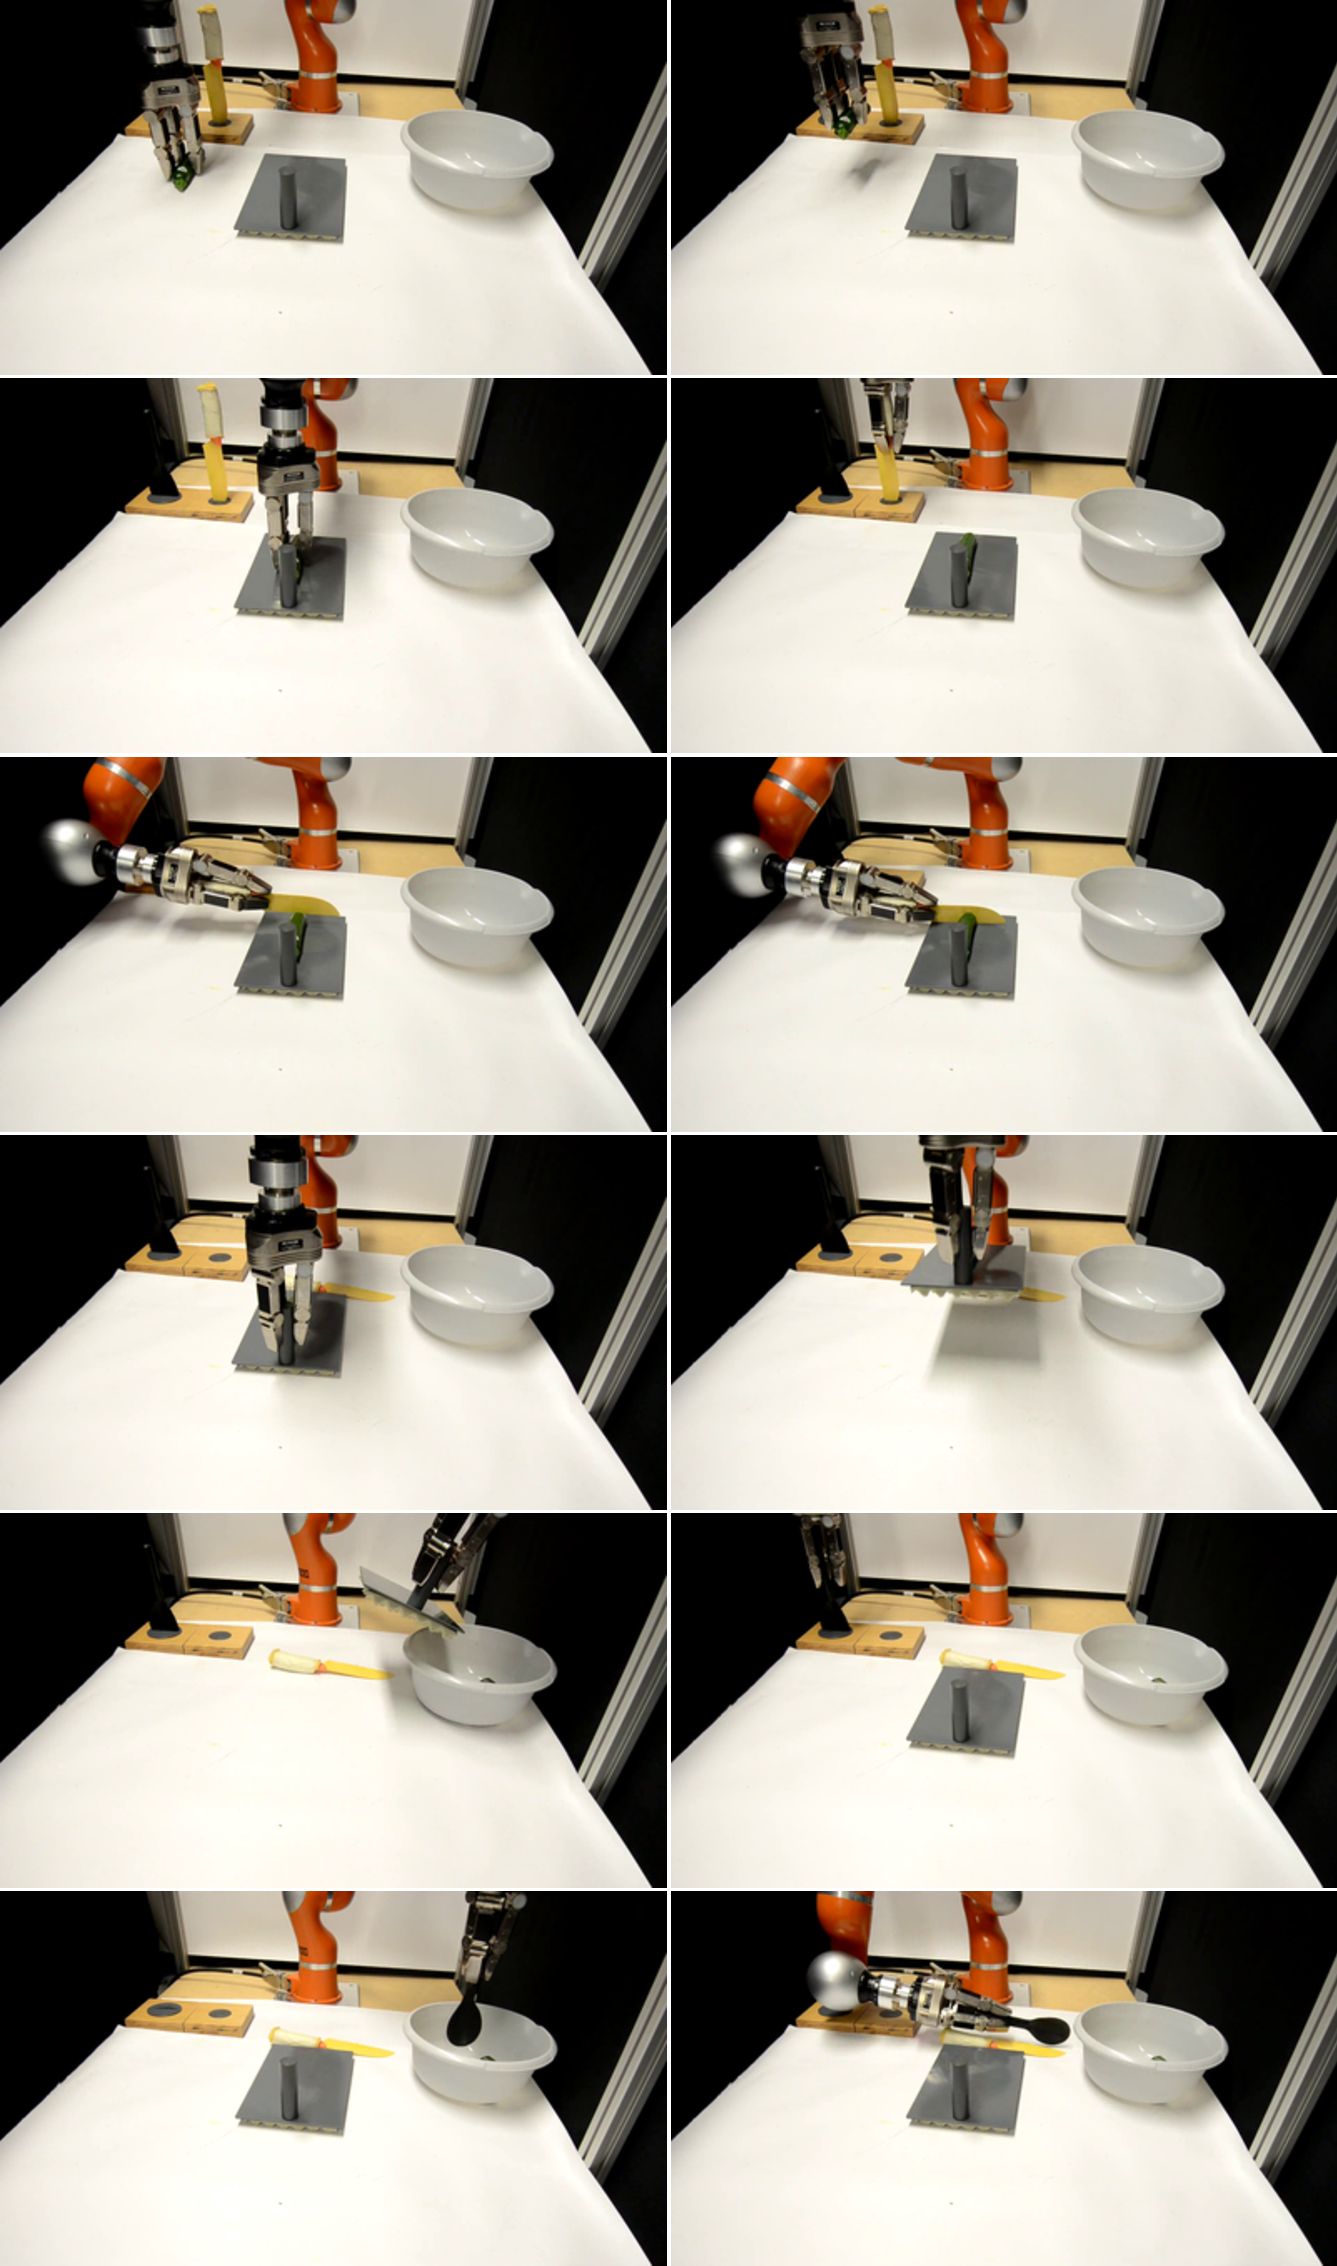
\includegraphics[scale=0.5]{./pdf/scenario_result.pdf}
      \caption{ Two instances of the put-on action, performed by our method, are shown with different objects and positions. 
The snapshots of the executed actions together with segmented images are shown (top) which indicate the real objects and relations.
The symbolic graph sequence (middle) and the SEC matrix (bottom) remain the same for both version.
}
      \label{fig:scenario_result}
\end{figure*}
Several actions have been executed in the proposed framework and are available in the library of actions.
The list of the actions are shown in table.\ref{tab:action_list}.
\begin{table}
% table caption is above the table
\caption{The list of actions in the library. The last two columns show example objects used in experiments.}
\label{tab:action_list}       % Give a unique label
% For LaTeX tables use
\begin{tabular}{llll}
\hline\noalign{\smallskip}
\# & Action Name & primary obj. & secondary obj. \\
\noalign{\smallskip}\hline\noalign{\smallskip}
1 & pick and place  & cup & - \\
2 & put-on-top & cup, cucumber & bucket, board \\ 
3 & take-down  & cup & bucket \\
4 & put-in  & cup & bucket \\
5 & cut  & knife & zucchini, cucumber, banana \\
6 & unload  & board & zucchini \\
7 & stir  & spoon & milk \\
8 & push  & box & - \\
9 & poke  & box & -\\
\noalign{\smallskip}\hline
\end{tabular}
\end{table}

The results of the put-on-top example are shown in Fig.\ref{fig:result_puton} for two instances.
For the results of other single actions please see our webpage \url{https://sites.google.com/site/aeinwebpage/actions}.

The actions can be chained to form more complex tasks, like making a salad.
A simple salad making scenario is created by chaining some of the actions in the library.
The scenario is as follows:
\begin{enumerate}
 \item Pick up a zucchini and place it on the cutting board (pick and place action)
 \item Grasp the knife and cut the zucchini (cutting action)
 \item Grasp the board and unload the zucchini pieces into a bowl (unload action)
 \item Grasp a spoon and stir into the bowl (stirring action)
\end{enumerate}

The result is shown in Fig.\ref{fig:scenario_result}.
The video of this scenario is also available in our webpage \url{https://sites.google.com/site/aeinwebpage/actions/videos}.











%%%%%%%%%%%%%%%%%%%%%%%%%%%%%%%%%%%%%%%%%%%%%%%%%%%%%%%%%%%%%%%%%%%%%%%%%%%%%%%%%%%%%%%%%%%%%%%%%%%%%%%%%%%%%
\section{Results}
\label{sec:results}

In this section, we will provide experimental results 

%%%%%%%%%%%%%%%%%%%%%%%%%%%%%%%%%%%%%%%%%%%%%%%%%%%%%%%%%%%%%%%%%%%%%%%%%%%%%%%%%%%%%%%%%%%%%%%%%%%%%%%%%%%%%
\subsection{Manipulation Action (ManiAc) Dataset}
\label{sec:maniacdataset}
 
%%%%%%%%%%%%%%%%%%%%%%%%%%%%%%%%%%%%%%%%%%%%%%%%%%%%%%%%%%%%%%%%%%%%%%%%%%%%%%%%%%%%%%%%%%%%%%%%%%%%%%%%%%%%%
\section{Discussion}
\label{sec:discussion}

The main contribution of our paper is a novel method for automatic semantic decomposition and recognition of long and complex manipulation sequences.  


%\newpage  %% needed for single columns
%\clearpage  %% needed for two columns
%%%%%%%%%%%%%%%%%%%%%%%%%%%%%%%%%%%%%%%%%%%%%%%%%%%%%%%%%%%%%%%%%%%%%%%%%%%%%%%%%%%%%%%%%%%%%%%%%%%%%%%%%%%%%
\section*{Appendix}
 

%%%%%%%%%%%%%%%%%%%%%%%%%%%%%%%%%%%%%%%%%%%%%%%%%%%%%%%%%%%%%%%%%%%%%%%%%%%%%%%%%%%%%%%%%%%%%%%%%%%%%%%%%%%%%
\begin{acknowledgements}
The research leading to these results has received funding from the European Community’s Seventh Framework Programme FP7/2007-2013 (Programme and Theme: ICT-2011.2.1, Cognitive Systems and Robotics) under grant agreement no. 600578, ACAT. 
\end{acknowledgements}





%%%%%%%%%%%%%%%%%%%%%%%%%%%%%%%%%%%%%%%%%%%%%%%%%%%%%%%%%%%%%%%%%%%%%%%%%%%%%%%%%%%%%%%%%%%%%%%%%%%%%%%%%%%%%
 

% BibTeX users please use one of
\bibliographystyle{spbasic}      % basic style, author-year citations
%\bibliographystyle{spmpsci}      % mathematics and physical sciences
%\bibliographystyle{spphys}       % APS-like style for physics
\bibliography{actionlib_journal}   % name your BibTeX data base


% Non-BibTeX users please use
%\begin{thebibliography}{}
%%
%% and use \bibitem to create references. Consult the Instructions
%% for authors for reference list style.
%%
%\bibitem{RefJ}
%% Format for Journal Reference
%Author, Article title, Journal, Volume, page numbers (year)
%% Format for books
%\bibitem{RefB}
%Author, Book title, page numbers. Publisher, place (year)
%% etc
%\end{thebibliography}

\end{document}
% end of file template.tex

